\begin{tframe}{Adversarial Training}

The method of training used for this case follows the one proposed by [1].

\vspace{0.1in}

The objective function is modified to include adversarial examples in the training phase:

$$ 	\tilde{J}(\theta, x, y) = \alpha J(\theta, x, y) + ( 1 - \alpha)J(\theta, x + \epsilon sign(\nabla_{x}J(\theta, x, y)), y) $$

\end{tframe}

\begin{tframe}{Adversarial Training}

\begin{center}
  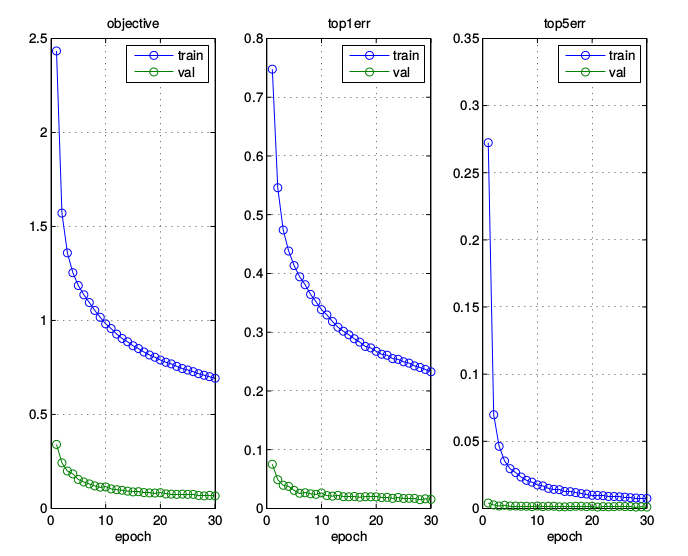
\includegraphics[width=0.7\textwidth]{img/train-adv.png}
	\label{train-mix} 
\end{center}

\end{tframe}

\begin{tframe}{Adversarial Training}

The tests were carried out as for the standard and mixed training.

\begin{table}[h]
\centering
\begin{tabular}{@{}lll@{}}
\toprule
                               & Clean & Adversarial \\ \midrule
Correctly Predicted            & 97.97 & 77.80       \\
Error                          & 2.03  & 22.20       \\
Confidence                     & 96.03 & 79.05       \\
Confidence Correctly Predicted & 96.69 & 82.55       \\
Confidence Error               & 64.23 & 66.79       \\ \bottomrule
\end{tabular}
\end{table}

\end{tframe}